\documentclass[]{article}
\usepackage{amsmath}
\usepackage{amsfonts}
\usepackage{bigstrut}

\usepackage[pdftex]{graphicx}	
\usepackage{float}
\usepackage{subfigure}

%opening
\title{IPP - Meta $\&$ THz (Sp-Su 2021)\\
	Notes}
\author{Xu Wentao 519370910166\\Li Chengfan 519370910172}

%begin
\begin{document}
	
	%abstract part
	\maketitle
	\begin{abstract}
		Metamaterials
		
	\end{abstract}
	
\clearpage
	\section*{Basics}
	\begin{enumerate}
		\item Why metamaterials?
		
		 $\textbf{Extreme Control}$ of EM waves, e.x. Invisibility, Ideal/Perfect Lens, etc.
		\item To be more specific, what is changed to achieve unusual control?
		
		The change of permitivity and permeativity, which leads to the change of refractive index (to be zero/negative), etc.
		\item The theories/models?
		\begin{enumerate}
			\item Generalized Snell's Law
			
			The wavefront of light through normal optical components such as lenses rely on $\textbf{gradual phase shift}$ accumulated along the optical path while an $\textbf{abrupt phase shift}$ is introduced as a new freedom of control. Still, Fermat's principal (shortest path) governs the light's propagation.
			
			The metasurface is extremely thin, even thinner than the wavelength. And thus, the gradual phase shift $\int_A^B d\phi (\vec{r})$ will be close to zero(or just zero) while the abrupt phase shift $\Phi(\vec{r_s})$ over the scale of wavelength can be introduced. It depends on coordinate $\vec{r_s}$ along the interface and the ultimate phase shift is calculated as $\Phi(\vec{r_s})+\int_A^B d\phi (\vec{r})$
			
			i)assume $\Phi$ being continuous, 
			\begin{align*}
				sin(\theta_t)n_t - sin(\theta_i)n_i &= \frac{\lambda_o}{2\pi}\frac{d \Phi}{dx}\\
				sin(\theta_r) - sin(\theta_i) &= \frac{\lambda_o}{2\pi n_r}\frac{d \Phi}{dx}\\
				arcsin(\pm \frac{n_t}{n_i} - \frac{\lambda_o}{2\pi n_r}\frac{d \Phi}{dx})  &= \theta_c , \quad n_t<n_i\\
				arcsin(1 - \frac{\lambda_o}{2\pi n_r}|\frac{d \Phi}{dx}|)  &= \theta_c'
			\end{align*}
		ii) Real-life: discreteness rather than continuity. Loss of energy rather than full transmission to reflection/refraction. So, we need numerical methods of Maxwell's equations.
		iii)Pictures about important parts:
	\begin{figure}[h]
		\begin{minipage}[t]{0.45\linewidth}
			\centering
			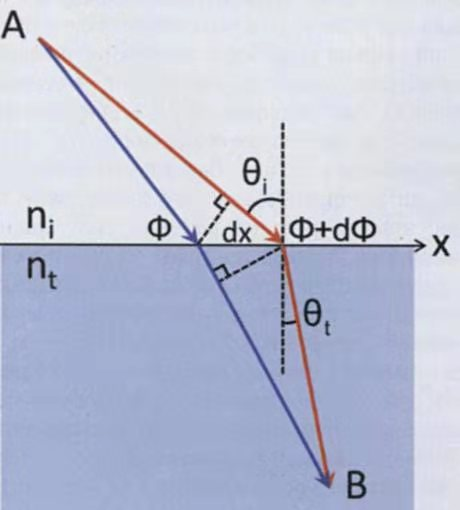
\includegraphics[width=5.5cm,height=5.5cm]{Fig/Snel0.jpg}
			\caption{Snell Foundamentals}
		\end{minipage}
		\begin{minipage}[t]{0.45\linewidth}        %图片占用一行宽度的45%
			\hspace{2mm}
			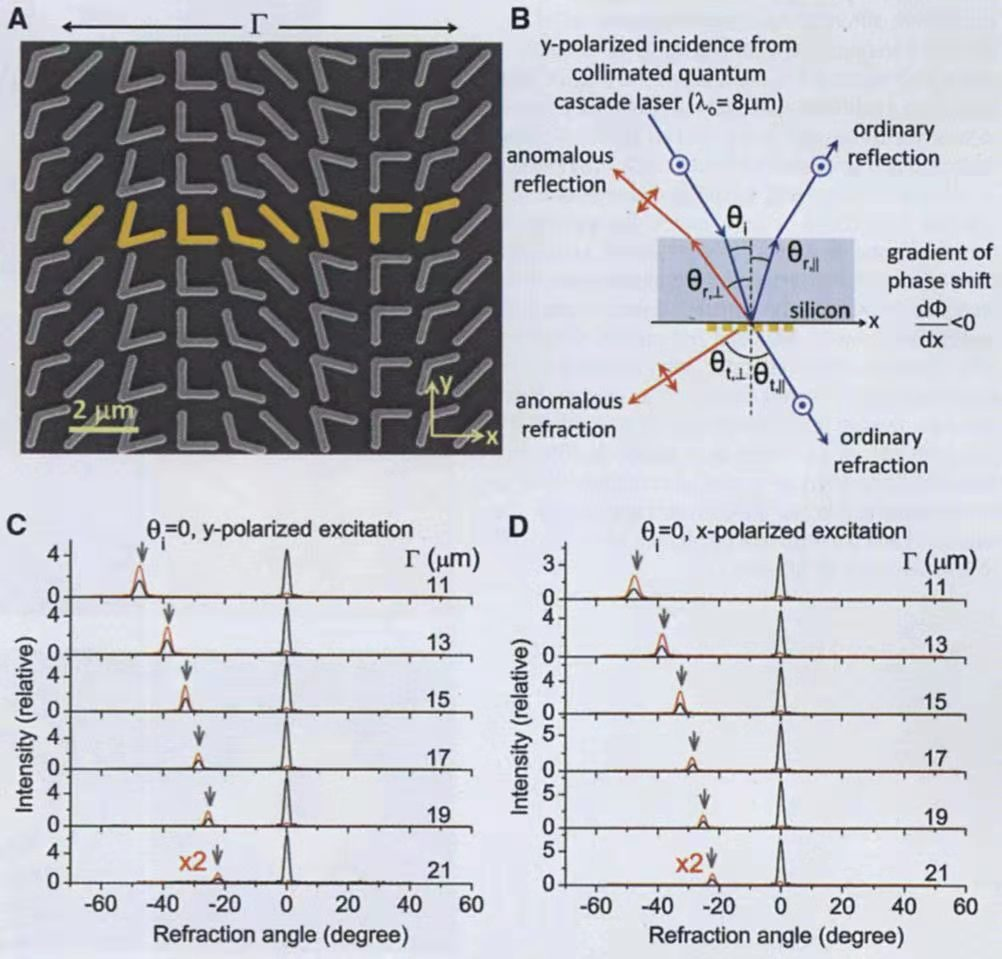
\includegraphics[width=5.5cm,height=5.5cm]{Fig/Snel1.jpg}
			\caption{Snell Sample Comparison}
		\end{minipage}
	\end{figure}
	\begin{figure}[h]
	\centering
		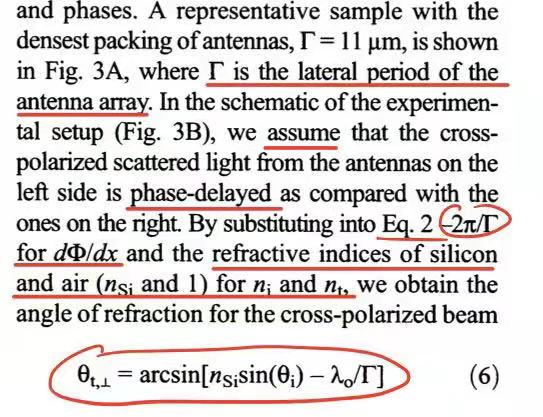
\includegraphics[width=6cm,height=4.5cm]{Fig/Snel2.jpg}
	\caption{Application of the snell's law}
	\end{figure}

		iii)How is this generalized snell's law used in papers?
		\begin{enumerate}
			\item gradient phase shift $\longrightarrow$ reflection in obligue angle. (general confirmation with simulation) by TJCui, Coding metamaterials.
			\item Find direction ($\Phi,\theta$) by assigning distributions of gradient phase responses. by L. Bao, Multi-Beam Forming and Controls.
			\item Just mention it and calculate the angle shift by 14.5 $^o$ with phase discontinuity. by L. Zhang, Space-time-coding digital metamaterials
			\item Extract effective refractive index $n^{eff}_r$ (conventional snell's law)
			\item phase pattern determines scattering directions of a beam on the surface. by Q. Ma Information metamaterial: bridging...
		\end{enumerate}
		
		iv)Conclusion for Snell's Law, not used widely, just taken as something for confirmation after the simulated outcome is present.
		
		\item Theory Background for Electromagnetic Principles:(not fully understandable)
			\begin{enumerate}
				\item General Maxwell Equations when viewing metamaterials as dielectrics/nonconductors:
				\begin{align*}
					\bigtriangledown \cdot D &= 0\\
					\bigtriangledown \cdot B &= 0\\
					\bigtriangledown \times E + \frac{\partial B}{\partial t} &= 0\\
					\bigtriangledown \times H + \frac{\partial D}{\partial t} &= 0\\
					\text{and}\quad D &= \epsilon E\\
					B &= \mu H
				\end{align*}
			Note that the electric permitivity and magnetic permeativity are dispersive right now, i.e. function of the frequency(complex function). $\epsilon(\omega)$, the solution $\frac{\epsilon(\omega)}{\epsilon_0}$ is called Kramers-Kronig relations(covered in HW of Vv286, forgotten).
			
			Anyway, the developed equations/solution travelling in x direction is in the form of
			\begin{align*}
				(\bigtriangledown^2 + \mu\epsilon\omega^2){E/B} &= 0\\
				E(x,t) = E_0 e^{i(kx-\omega t)}&\\
				B(x,t) = B_0 e^{i(kx-\omega t)}&\\
				k = \sqrt{\epsilon\mu}\omega&
			\end{align*}
		k is the wave number, sometimes called as spatial modulation frequency $\beta$ when the environment is changed, so is $\omega$.
		
		Next, phase velocity, refractive index and wave impedance are introduced as
		\begin{align*}
			v &= \frac{\omega}{k} = \frac{1}{\epsilon \mu} = \frac{c}{n}\\
			 n &= \sqrt{\frac{\mu\epsilon}{\mu_0\epsilon_0}} = \sqrt{\mu_r}{\epsilon_r}\\
			Z &= \frac{E_0}{H_0} = \sqrt{\frac{\mu}{\epsilon}} = \frac{\mu_r}{\epsilon_r}Z_0 = \zeta Z_0
		\end{align*}
		\item Negative Index, how is that happening?
		
		When taking square root, we are not taking negative because conventionally the materials are right-handed/positive($\epsilon>0,\mu>0$).
		
		However, reconstruct complex $epsilon_r$ and $\mu_r$ and find $\epsilon_r = e^{i\Phi_{\epsilon}}, \mu_r = e^{i\Phi_{\mu}}$ where the phases $\Phi_{\epsilon}$ and $\Phi_{\mu}$ are between pi/2 and pi, finding n to be negative.
		
		\item Propagation
		
		Reduce the equations to 
		\begin{align*}
			k \times E &= \omega \mu H\\
			k \times H &= -\omega\epsilon E\\
			S &= E \times H
		\end{align*}
		where S is the poynting vector telling the energy flux, in anti-parallel with the wave vector k in left-handed materials.
		
		\item Single-negative ingredient propagation
		
		It is decaying wave since k's imaginary part is decaying.
		\end{enumerate}
	
	\clearpage
		\item Space-Time Modulation
		\begin{figure}[h]
			\centering
			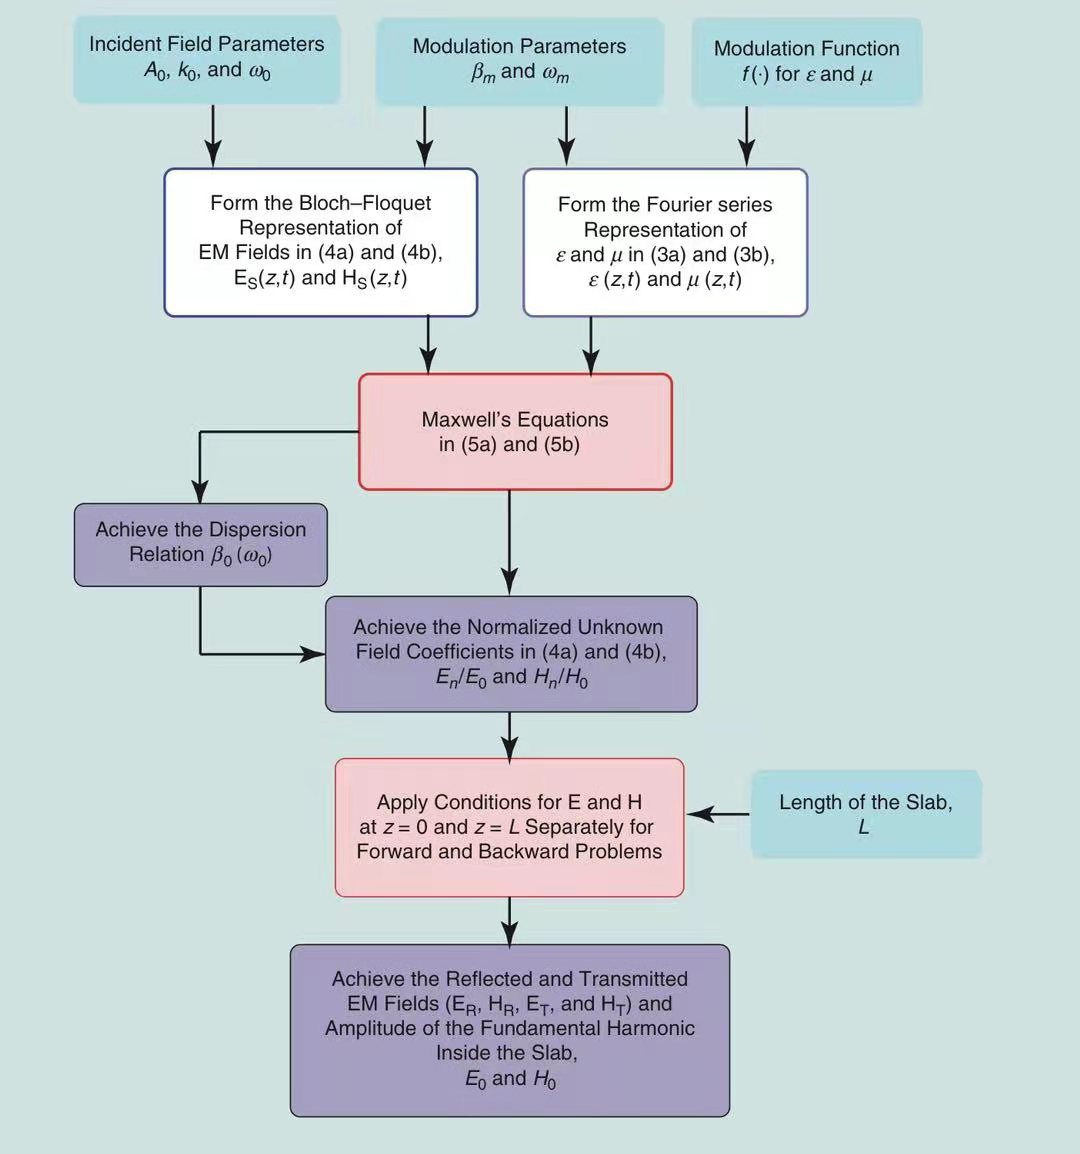
\includegraphics[width=12cm,height=14cm]{Fig/SpacTimeModu.jpg}
			\caption{Find the scattered solution for STM slab}
		\end{figure}
	
		Equations mentioned:
		\begin{align*}
			\beta_m &= \frac{\omega_m}{\nu_m} = \frac{\omega_m}{\gamma\nu_b}\\
			\epsilon(z,t) &= \sum\limits_{k = -\infty}^{\infty}\tilde{\epsilon_k}e^{-jk(\beta_mz-\omega_mt)} \quad (3a)\\
			\mu(z,t) &= \sum\limits_{k = -\infty}^{\infty}\tilde{\mu_k}e^{-jk(\beta_mz-\omega_mt)} \quad (3a)\\
			E_s(z,t) &= \hat{x} e^{-i(\beta_0z - \omega_0t)}\sum\limits_{n = -\infty}^{\infty}E_ne^{in(\beta_mz-\omega_mt)} \quad (4a)\\
			H_s(z,t) &= \hat{y} e^{-i(\beta_0z - \omega_0t)}\sum\limits_{n = -\infty}^{\infty}H_ne^{in(\beta_mz-\omega_mt)} (4b)\\
			\frac{\partial E_x(z,t)}{\partial z} &= -\frac{\partial [\mu(z,t)H_y(z,t)]}{\partial t} \quad (5a)\\
			\frac{\partial H_y(z,t)}{\partial z} &= -\frac{\partial [\epsilon(z,t)E_x(z,t)]}{\partial t} \quad (5b)
		\end{align*}
		
		\end{enumerate}
	
	\end{enumerate}
	\clearpage
	\section*{Papers $\&$ Concepts}
	\begin{enumerate}
		\item 2003 Kuester "generalized sheet transition conditions (GSTCs)':
		\begin{enumerate}
			\item How to derive conditions: replace discrete distribution of scatters with continuous one. Similar to Clausius–Mossotti–Lorenz–Lorentz procedure for determining the dielectric constant of a volume distribution of small
			scatterers.
			\item GSTCs: an equivalent transition
			(boundary) condition for the specular interaction of electromagnetic waves with a surface of electrically small scatterers.
			\item Scatters: characterized completely by
			their electric and magnetic polarizabilities and their density of
			distribution in the surface.
			\item metafilm $\approx$ 2-D metamaterial: have certain desired reflection and transmission properties (e.g., total reflection or total transmission).
			\item Importance: Generalized functional dependence of the polarizability densities to
			the reflection and transmission properties of the surface, realizing controllable surfaces.
			\item Applicable to: metafilms
			located in a homogeneous(unifromly same) medium.
			\item Conclude: Concept generation, the output condition is not easy for calculation. Also, it is just mentioned as background, not as actual calculation steps. So, now should focus on generalized snell's law and other practical formulas that have been widely adopted.
		\end{enumerate}
		
	\end{enumerate}
	
	
	
	\section*{Structure and theroretical background}
	\subsection*{Simplest 1-bit case}
	\begin{figure}[H]
		\centering
		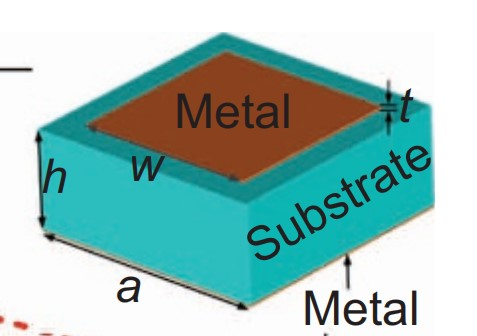
\includegraphics[scale=0.65]{Fig/1.jpg}
		\caption{The Structure}
	\end{figure}
	\par And we have the following function of scattering field in a spherical coordinate system.
	\begin{figure}[H]
		\centering
		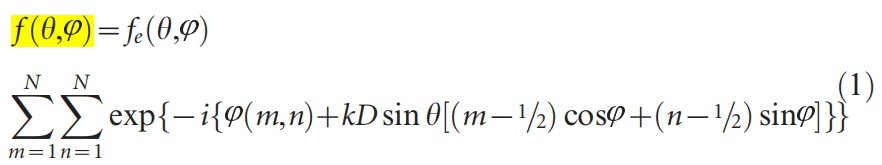
\includegraphics[scale=0.65]{Fig/2.jpg}
	\end{figure}
	\par More information
	\begin{enumerate}
		\item Digital control
			\par 0-0  width of the metal: 3.75mm
			\par 1-$\pi$   width of the metal: 4.8mm
		\item Frequency 
			\par 8.1 - 12.7 GHz
		\item Control of the amplitude and phase
			\par Can't achieve separate control
	\end{enumerate}

	\subsection*{Other Passive Structures}
		\begin{figure}[H]
		\centering
		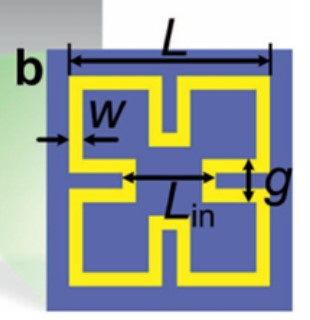
\includegraphics[scale=0.8]{Fig/10.jpg}
	\end{figure}
	
	\begin{figure}[H]
		\centering
		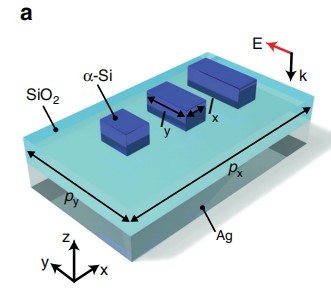
\includegraphics[scale=0.8]{Fig/11.jpg}
	\end{figure}
	
	\begin{figure}[H]
		\centering
		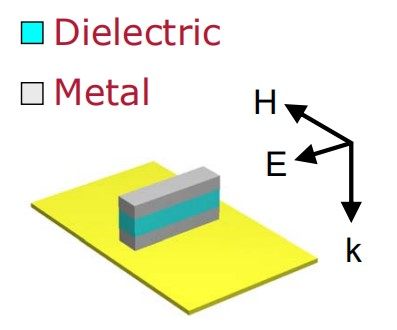
\includegraphics[scale=0.8]{Fig/12.jpg}
	\end{figure}

	\subsection*{From passive to active}
	\begin{figure}[H]
		\centering
		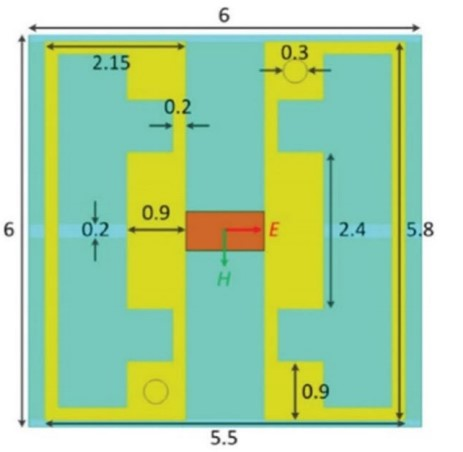
\includegraphics[scale=0.8]{Fig/3.jpg}
	\end{figure}
	
	\subsection*{Simulation}
	\par The simulation result from the paper:
	\begin{figure}[H]
		\centering
		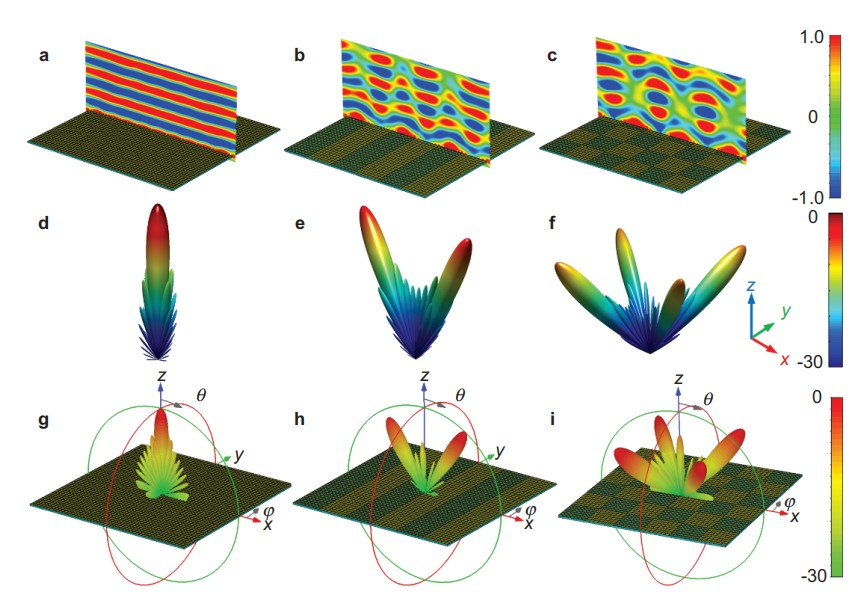
\includegraphics[scale=1]{Fig/4.jpg}
		\caption{Result}
	\end{figure}

	\par Our simlation results using Matlab.
	\begin{figure}[H]
		\centering
		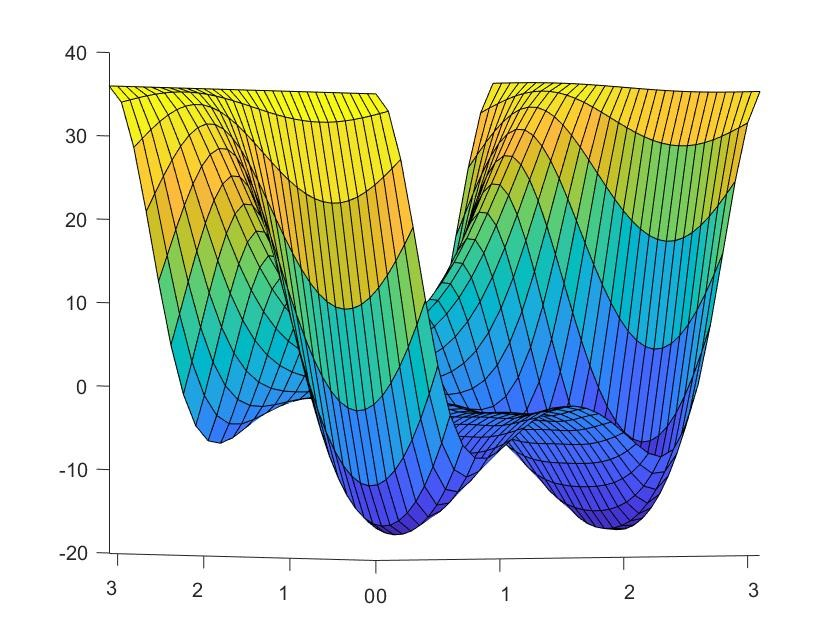
\includegraphics[scale=0.3]{Fig/5.jpg}
		\caption{000000/000000}
	\end{figure}

	\begin{figure}[H]
		\centering
		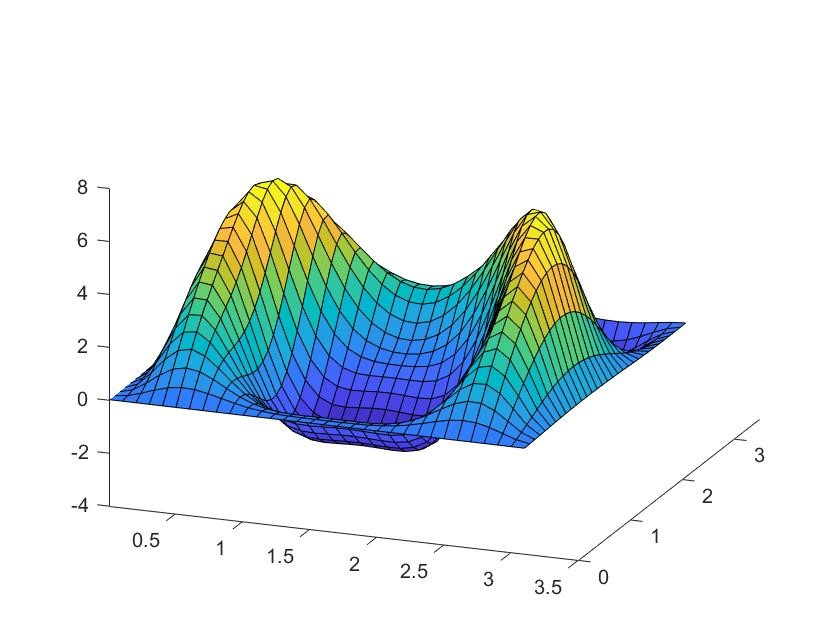
\includegraphics[scale=0.3]{Fig/6.jpg}
		\caption{010101/010101}
	\end{figure}
	
	\begin{figure}[H]
		\centering
		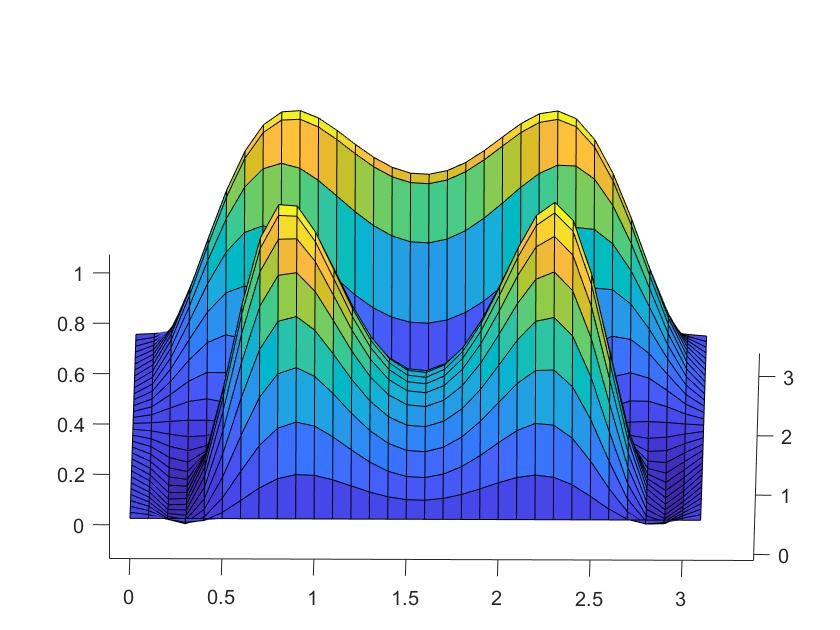
\includegraphics[scale=0.3]{Fig/7.jpg}
		\caption{010101/101010}
	\end{figure}


	\subsection*{Radar Cross Section}
	
		\begin{figure}[H]
		\centering
		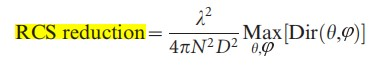
\includegraphics[scale=0.8]{Fig/8.jpg}
	\end{figure}
	
	\begin{figure}[H]
		\centering
		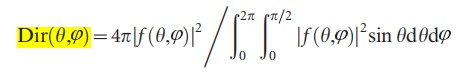
\includegraphics[scale=0.8]{Fig/9.jpg}
	\end{figure}

	\par One of the aim is minimize the RCS.
	
	\subsection*{C-shape}
	\par From "Multi-Beam Forming and Controls by Metasurface With Phase 
	and Amplitude Modulations (002)"
	
	\par Based on the above conclusion, the regulation mechanism of amplitude and phase are further improved.
	
	\begin{figure}[H]
		\centering
		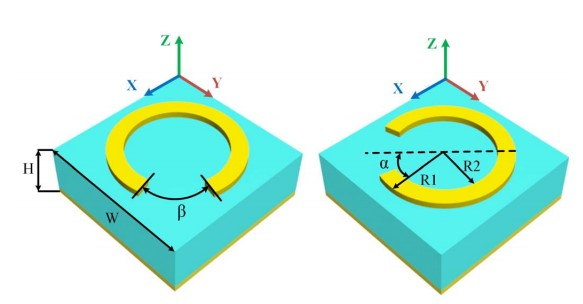
\includegraphics[scale=0.65]{Fig/13.jpg}
		\caption{C-shape from 002}
	\end{figure}
	\par $\beta$ for phase, $\alpha$ for amplitude.
	\par When amplitude can be modified, the introduced new coefficient is calculated by
	
	\begin{figure}[H]
		\centering
		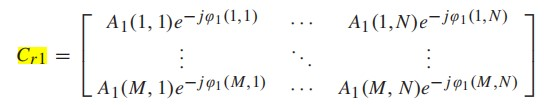
\includegraphics[scale=0.8]{Fig/14.jpg}
	\end{figure}


	\subsection*{More on C-shape}
	\begin{figure}[H]
		\centering
		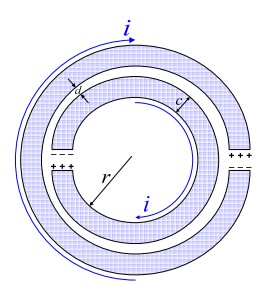
\includegraphics[scale=0.8]{Fig/15.jpg}
	\end{figure}

	\begin{figure}[H]
		\centering
		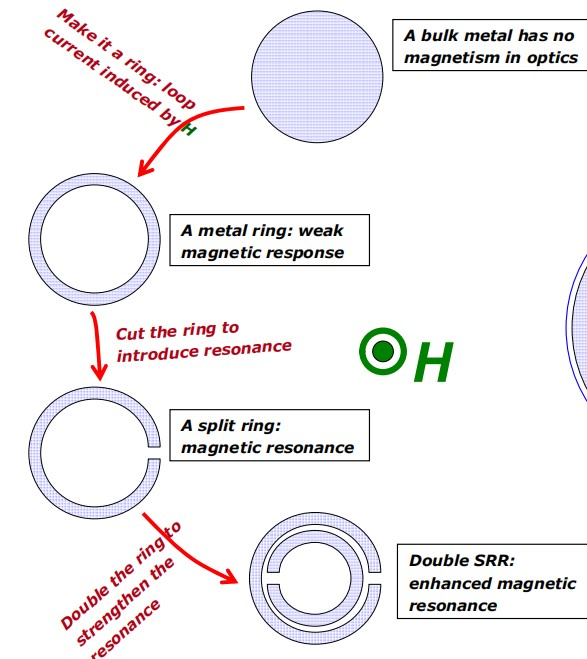
\includegraphics[scale=0.8]{Fig/16.jpg}
	\end{figure}

	\par Resonance can improve the effect of switch on/off.
	
	\begin{figure}[H]
		\centering
		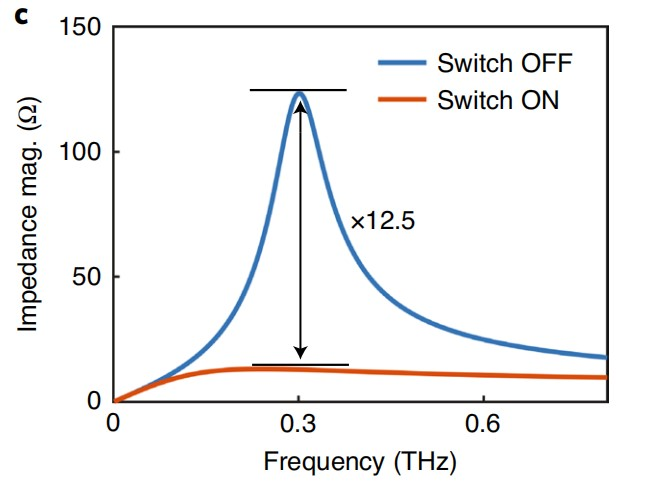
\includegraphics[scale=0.8]{Fig/17.jpg}
	\end{figure}
	
	\begin{figure}[H]
		\centering
		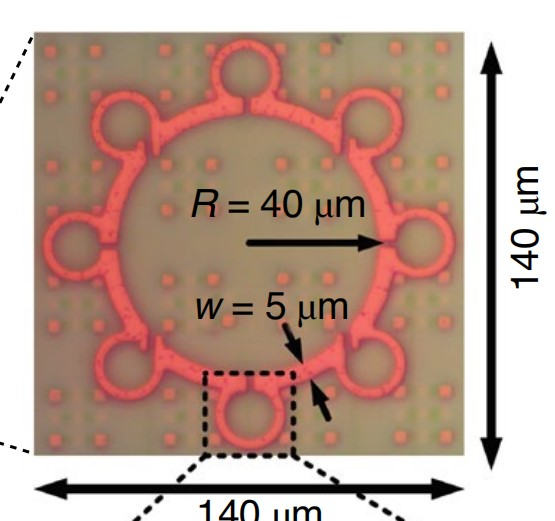
\includegraphics[scale=0.65]{Fig/18.jpg}
	\end{figure}


	\subsection*{Space-time-coding digital metasurfaces}
	\begin{figure}[H]
		\centering
		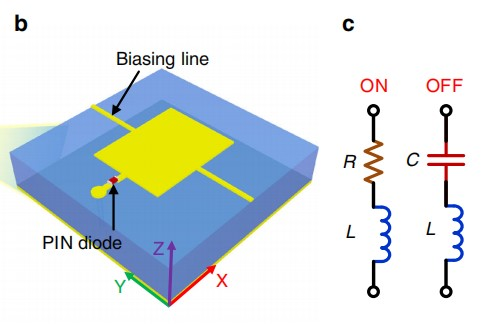
\includegraphics[scale=0.8]{Fig/19.jpg}
	\end{figure}

	\subsection*{Multi-layer}
	\begin{figure}[H]
		\centering
		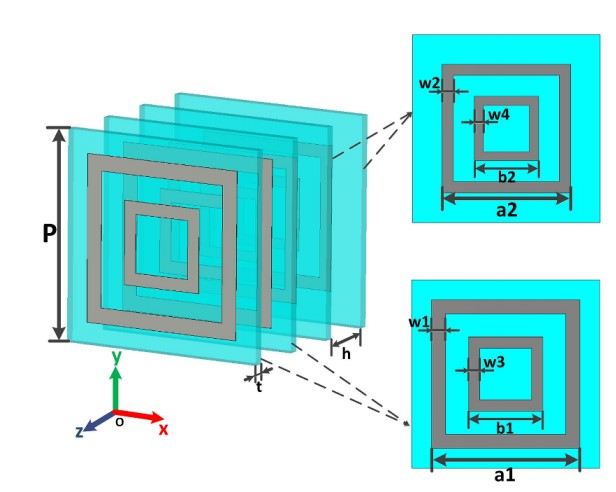
\includegraphics[scale=0.8]{Fig/20.jpg}
	\end{figure}

	\par Information
	\par 10GHz
	\par 00  \qquad  0,0.1 \qquad  0
	\par 01  \qquad  0.3,0.4 \qquad  -90
	\par 10  \qquad  0.6,0.7  \qquad -180
	\par 11  \qquad  0.85,0.95 \qquad  -270
\end{document}